\documentclass[a4paper,oneside]{memoir}
\usepackage{listings}%
\usepackage{xcolor}
\usepackage{hyperref}
\lstset{%
    backgroundcolor=\color{yellow!20},%
    basicstyle=\small\ttfamily,%
    numbers=none, numberstyle=\tiny, stepnumber=2, numbersep=5pt,%
    }%

\lstset{emph={%  
    PARAM%
    },emphstyle={\color{blue}\bfseries},%
    morekeywords={filename},
    keywordstyle={\color{red}\ttfamily}
}%

\usepackage{fourier} % or what ever
\usepackage[scaled=.92]{helvet}%. Sans serif - Helvetica
\usepackage{color,calc}
\newsavebox{\ChpNumBox}
\definecolor{ChapBlue}{rgb}{0.00,0.65,0.65}
\makeatletter
\newcommand*{\thickhrulefill}{%
  \leavevmode\leaders\hrule height 1\p@ \hfill \kern \z@}
\newcommand*\BuildChpNum[2]{%
  \begin{tabular}[t]{@{}c@{}}
    \makebox[0pt][c]{#1\strut}  \\[.5ex]
    \colorbox{ChapBlue}{%
      \rule[-10em]{0pt}{0pt}%
      \rule{1ex}{0pt}\color{black}#2\strut
      \rule{1ex}{0pt}}%
  \end{tabular}}
\makechapterstyle{BlueBox}{%
  \renewcommand{\chapnamefont}{\large\scshape}
  \renewcommand{\chapnumfont}{\Huge\bfseries}
  \renewcommand{\chaptitlefont}{\raggedright\Huge\bfseries}
  \setlength{\beforechapskip}{0pt}
  \setlength{\midchapskip}{26pt}
  \setlength{\afterchapskip}{40pt}
  \renewcommand{\printchaptername}{}
  \renewcommand{\chapternamenum}{}
  \renewcommand{\printchapternum}{%
    \sbox{\ChpNumBox}{%
      \BuildChpNum{\chapnamefont\@chapapp}%
      {\chapnumfont\thechapter}}}
  \renewcommand{\printchapternonum}{%
    \sbox{\ChpNumBox}{%
      \BuildChpNum{\chapnamefont\vphantom{\@chapapp}}%
      {\chapnumfont\hphantom{\thechapter}}}}
  \renewcommand{\afterchapternum}{}
  \renewcommand{\printchaptertitle}[1]{%
    \usebox{\ChpNumBox}\hfill
    \parbox[t]{\hsize-\wd\ChpNumBox-1em}{%
      \vspace{\midchapskip}%
      \thickhrulefill\par
      \chaptitlefont ##1\par}}%
}
\chapterstyle{BlueBox}

\setlength\afterchapskip {\onelineskip }
\setlength\beforechapskip {\onelineskip }

%\setlength{\oddsidemargin}{0.03\paperwidth} 
%\setlength{\evensidemargin}{0.03\paperwidth}
%\setlength{\textwidth}{0.7\paperwidth}
%\setlength{\voffset}{0pt}

%\usepackage{anysize}
%\marginsize{2.25cm}{2cm}{}{1,25 cm}
\setlrmarginsandblock{3cm}{2.5cm}{*}
\setulmarginsandblock{2.5cm}{2.5cm}{*}
\checkandfixthelayout

\usepackage{graphicx}
\usepackage{float}
\graphicspath{{./img/}}
\DeclareGraphicsExtensions{.pdf,.jpeg,.png}


\begin{document}

\let\clearforchapter\par % cheating, but saves some space
\chapter{The TLUT tool flow: An introduction}

The TLUT tool flow is a tool flow that generates FPGA configurations. Its biggest difference with the traditional FPGA flow is the use of a new technology mapper, the TLUT mapper. The TLUT tool flow was developed to implement Dynamic Circuit Specialization (DCS) on FPGAs. A DCS implementation of an application specializes its circuit for the current values of a number of specific inputs, called parameters. This specialized circuit is smaller, and in some cases faster, than the original circuit. However, it is only correct for one set of parameter values. Each time the parameters change value, a new specialized circuit is generated. This new specialized circuit is then loaded into the FPGA using partial run-time reconfiguration.\\

The TLUT tool flow offers an efficient implementation of DCS because it uses the concept of parameterized configurations. A parameterized configuration is a configuration in which some bits are expressed as Boolean functions of the parameters. Before the FPGA can be configured, the parameter values are used to evaluate the Boolean functions. This generates the specialized configuration. Several papers on the academic underpinnings of the TLUT tool flow are listed in the wiki of this project or are contained in the documentation directory. There you can also find more information on our current research on extending and improving the TLUT tool flow. The TLUT tool flow itself and how to use it, is described in much more detail in this user guide.

\section{What can I do with this tool flow?}
First, you can evaluate our adapted TLUT technology mapper. 
This  allows you to compare its results with a conventional technology mapper and see for yourself if Dynamic Circuit Specialization can be used to optimize your application. 
We have included a framework to make this comparison very easy. 
The following pages provide clear examples and show how to adapt the framework for you own uses.

Second, our tool flow has been integrated with the Xilinx FPGA tool flow so that you can perform DCS on a commercial Virtex 2 Pro FPGA.
A number of examples that you can run right away on the XUP V2P board are included in this repository. 
Information on creating your own project is also included in this document.
We are currently working on extending this tool flow to more modern FPGAs, such as the Virtex 5 or 6.

\section{Contact us}
The TLUT tool flow is released by Ghent University, ELIS department, Hardware and Embedded Systems (HES) group (\href{http://hes.elis.ugent.be}{\emph{http://hes.elis.ugent.be}}).

If you encounter bugs, want to use the TLUT tool flow but need support or want to tell us about your results, feel free to contact us.
We can be reached at \href{mailto:hes@elis.ugent.be}{\emph{hes@elis.ugent.be}}.

\section{Referencing the TLUT tool flow}
If you use the TLUT tool flow in your work, please reference in your publications the following paper:

\emph{Karel Bruneel, Wim Heirman, and Dirk Stroobandt. 2011. ``Dynamic Data Folding with Parameterizable FPGA Configurations.'' ACM Transactions on Design Automation of Electronic Systems 16 (4).}

You may also refer to one of our others papers if you think it is more related.

\section{Contents of this document}
Chapter~\ref{sec:setup}: \emph{Setup}: The setup manual\\
Chapter~\ref{sec:standalone_flow}: \emph{Standalone TLUT tool flow}: The manual for running your own experiments without implementation on an FPGA\\
Chapter~\ref{sec:xilinx_flow}: \emph{Xilinx-integrated TLUT tool flow}: The manual for creating your own DCS project using the Xilinx XUPV2P board\\
Chapter~\ref{sec:contents}: \emph{Contents}: Description of the contents of this package\\

\clearpage
\chapter{Setup}\label{sec:setup}
\begin{lstlisting}
> make
\end{lstlisting}
This downloads and builds the dependencies listed below, builds the TLUT technology mapper and creates a `source' file which sets environment variables. 
Make sure you agree with the respective licences of the dependencies before running make. 

Set your environment variables using:
\begin{lstlisting}
> . source
\end{lstlisting}

Section~\ref{sec:tlut_testing} explains how to test the TLUT tool flow, while in Section~\ref{sec:xilinx_testing} you can find information on how to test the integration with the Xilinx tool flow and the XUPV2P board.

\section{Dependencies}
\begin{itemize}
\item Dependencies to be provided by the user:
\begin{itemize}
\item A UNIX operating system (tools used: gcc, bash, minicom, curl, stty, \dots)
\item Quartus II (tested with Web Edition version 11, Web Edition v12 may work but is not supported), Altera Corporation, \url{http://www.altera.com}
\item Java (tested with version 1.6.0), Oracle, \url{http://www.java.com}
\item Python 2.7, \url{http://www.python.org}
\item Xilinx Design Suite 9.1 (tested with version 9.1.02), Xilinx Inc., \url{http://www.xilinx.com}\\
Version 9.1 is old, but it is unlikely that other versions will work.
\item A Xilinx XUP Virtex-II Pro Development System (XUPV2P board)\\
Xilinx Platform Builder and the XUPV2P board are only required for implementation of DCS on a commercial FPGA. 
\end{itemize}
\item Dependencies automatically downloaded and installed:
\begin{itemize}
\item Aiger 1.9.4, JKU Institute for Formal Models and Verification, \url{http://fmv.jku.at/aiger}
\item ABC (version 810ba683c042, 5 October 2012), Berkeley Logic Synthesis and Verification Group, \url{http://www.eecs.berkeley.edu/\~alanmi/abc}
\item RapidSmith 0.5.1, BYU RapidSmith Projec,  \url{http://rapidsmith.sourceforge.net}
\item Hessian 4.0.7, Caucho Technology, \url{http://hessian.caucho.com}
\end{itemize}
\end{itemize}

\clearpage
\chapter{Standalone TLUT tool flow}\label{sec:standalone_flow}
The standalone TLUT tool flow can be used to evaluate the impact of DCS on your design. This tool flow will map your annotated VHDL or Verilog design and tell how much smaller or faster (LUT depth) your design can become when using parameterized configurations.

A number of examples are included in the `examples' directory that you can run using the included Python scripts.
E.g.
\begin{lstlisting}
> cd examples/treeMult4b
> ./treeMult4b.py
\end{lstlisting}

\section{Testing}\label{sec:tlut_testing}
Your installation of the TLUT tool flow can be tested using the script in the directory `tests'.
\begin{lstlisting}
> cd tests
> ./examples_test.sh
\end{lstlisting}
If you encounter errors, troubleshooting information can be found in Section~\ref{sec:tlut_troubleshooting}.


\section{Creating your own project: A step-by-step approach}\label{sec:step_by_step}
Below, we have provided a step-by-step approach to set up your own Python script starting from the \emph{treeMult4b} example:
\begin{enumerate}
\item Make a folder for your design and copy the treeMult4b folder from the examples directory. You need at least the files \emph{abc.rc} and \emph{treeMult4b.py}
\begin{lstlisting}
> mkdir yourDesign
> cp -r examples/treeMult4b/* yourDesign/
\end{lstlisting}
\item Replace treeMult4.vhd by copying your VHDL/Verilog files, describing your design, into the \emph{yourDesign}-folder
\begin{lstlisting}
> rm treeMult4b.vhd
\end{lstlisting}
\item Annotate the parameters in your top level VHDL/Verilog file.

Any input signal, or combination of input signals, of your top level module can be chosen as parameter. Preferably the designer will choose the slowly changing input signals as parameters, because a change in the value of the parameters results in a reconfiguration of the FPGA. Different combinations can be tested easily by changing the annotations. In the following example a simple multiplexer is described in VHDL and the `sel' input signal is annotated as a parameter.
\lstset{language=VHDL}
\begin{lstlisting}
entity multiplexer is
port(
  --PARAM
  sel : in  std_logic_vector(1 downto 0);
  --PARAM
  in  : in  std_logic_vector(3 downto 0);
  out : out std_logic
);
end multiplexer;

architecture behavior of multiplexer is
begin
  out <= in(conv_integer(sel));
end behavior;
\end{lstlisting}
The Verilog annotations are quite similar. The following Verilog example, a simple multiplier, can be found in the examples folder;
\lstset{language=Verilog}
\begin{lstlisting}
module mult(x,y,z);
parameter N = 16;
input [N-1:0] x;
//PARAM
input [N-1:0] y;
//PARAM
output [2*N-1:0]z;
assign z = x * y;
endmodule
\end{lstlisting}
 
\item Modify the Python script
\begin{lstlisting}
> mv treeMult4b.py yourDesign.py
> nano yourDesign.py
\end{lstlisting}
Edit the 6th line, in which the \emph{run} function is called, according to the documentation in Section~\ref{sec:run_function}. The most important change you have to make is filling in the name of the VHDL file of your design.

\item Run the modified Python script
\begin{lstlisting}
> ./yourDesign.py
\end{lstlisting}
\item \label{sec:check_par}Check the `.par' file in the work directory, to ensure the parameters were correctly recognised. It should list all the signal names of the parameters, i.e. one for each line of a bus signal. 
The tool for extracting parameters from VHDL and Verilog is still limited and can not yet parse all VHDL/Verilog constructs.
\item Analyze the results. As an example, the output of the Python script of the treeMult4b project is given;

\begin{lstlisting}
Stage: TLUT mapper
Luts (TLUTs)     depth     check
12 (12)          1         PASSED    
Stage: SimpleMAP
Luts             depth     check     
67               10        PASSED    
Stage: ABC fpga
Luts             depth     check     
67               10        PASSED 
\end{lstlisting}

The first column shows the number of LUTs in each mapping solution. These can be compared directly and represents the number of K-LUTs needed to implement the design. In this case, the TLUT mapper needs 12 LUTs, and SimpleMAP and ABC's fpga need 67.

SimpleMAP and ABC fpga both perform mapping for a conventional, not parameterised, configuration. The same results could be expected for both tools because they implement basically the same algorithm. However, ABC fpga contains some optimisations, such as `area recovery', which haven't been (completely) implemented in SimpleMAP. While the number of LUTs may differ between the two tools, you can expect the depth to be always equal.

The number between brackets `()' is only relevant for the TLUT mapper. It shows the number of LUTs that will actually be reconfigured at run-time. We call these LUTs TLUTs. In this case all 12 of the LUTs are TLUTs and will be reconfigured at run-time.

The third column shows the depth of each mapping solution. This is the number of LUTs in the longest path, a measure for the speed of the circuit. 

Finally, column 4 shows if the mapping solution has passed the equivalence test. This check is performed to see if the resulting circuit still has the same functionality as the original input.

% Hier de verschillen tussen simpleMap en abc bespreken of later pas in hoofdstuk 4?

\end{enumerate}


\section{The $run$ function}\label{sec:run_function}
To test the TLUT mapper on your own design (described in VHDL or Verilog), import the \emph{run} function from \emph{fast\_tlutmap} in your own Python script and call it with the following arguments:
\begin{lstlisting}
run(module, submodules, K, performCheck, verboseFlag)
\end{lstlisting}
\begin{itemize}
\item \textbf{module} - String\\
The location of the top level of your design. If your design consists of only one VHDL/Verilog module, then you only have to pass the location of this module as the first argument and you can ignore the second argument.

E.g. run('yourDesign.vhd')

\item \textbf{submodules} - list of Strings - \textit{optional}\\
If your design consists of a top level module and several submodules, you can add a list of submodules here, for example if you have one top level module and two submodules.

E.g. run('yourTopLevelModule.vhd', ['yourFirstSubModule.vhd', 'yourSecondSubModule.vhd'])

\item \textbf{K} - integer - \textit{default 4}\\
You can choose the number of inputs a LookUp Table has on your target FPGA

E.g. run('yourDesign.vhd', 6)
or run('yourDesign.vhd', K=6)

\item \textbf{performCheck} - boolean - \textit{default True}\\
When checks are turned on, the resulting mapping is verified using a miter and satisfiability solver. This ensures that the mapped circuit implements the same functionality as the input circuit.

E.g. run('yourDesign.vhd', 6, True)\\
or run('yourDesign.vhd', performCheck=False)

\item \textbf{verboseFlag} - boolean - \textit{default False}\\
This activates the verbose mode in which more information gets printed regarding the execution of the flow.

E.g. run('yourDesign.vhd', 6, True, True)\\ or run('yourDesign.vhd', verboseFlag=True)
\end{itemize}


\section{Advanced}
It is also possible to start from an `.aag' or `.blif' file. As a reference for this we provide examples \emph{AES} and \emph{tripleDES}. 
Advanced experiments can be set up by copying \emph{fast\_tlutmap} and using this file as a template for your experiment.

\section{Troubleshooting}\label{sec:tlut_troubleshooting}
Try running one of the examples in the `examples' folder to verify that your environment is set up correctly.\\

These are a few common errors and their solution:
\begin{itemize}
\item \emph{Throws ``Python ImportError: No module named fast\_tlutmap'' (or others):}\\
The environment variables probably aren't set up correctly. Try running `. source' in the main directory. 
If you have moved the main directory, the paths in the `source' file are no longer correct. Update it using `make source' and do `. source' again.

\item \emph{Throws ``java.lang.OutOfMemoryError'':}\\
The Java technology mappers don't have enough memory available. Try to use the \emph{setMaxMemory} function. It can be imported from the \emph{fast\_tlutmap} Python script and should be called before the \emph{run} function. This function sets the maximum memory usage for the Java tools in megabytes.
\lstset{language=python}
\begin{lstlisting}
from fast_tlutmap import run, setMaxMemory

setMaxMemory(4096)
run('treeMult4b.vhd', K=4, performCheck=True, verboseFlag=False)
\end{lstlisting}

\item \emph{The number of TLUTs is 0, or the reduction in number of LUTs is lower than expected:}\\
Check if all parameters were correctly extracted from your VHDL/Verilog. See Section~\ref{sec:step_by_step}, step~\ref{sec:check_par}.
\end{itemize}


\clearpage
\chapter{Xilinx-integrated TLUT tool flow}\label{sec:xilinx_flow}
The Xilinx-integrated TLUT tool flow can be used to build an application with DCS on the XUPV2P board (Currently only designs in VHDL, not Verilog).
A number of examples are included in the `examples' directory.
\begin{itemize}
\item `examples/xorExample/xps'
\item `examples/xorExample/xps\_mi'
\item `examples/treeMult4b/xps'
\end{itemize}

\section{Testing}\label{sec:xilinx_testing}
This section explains how you can run  all these examples to test your setup.

First, connect your XUPV2P board to the computer using a USB cable (for bitstream configuration) and a serial cable (for debugging).
Then, open each of the projects `examples/xorExample/xps',  `examples/xorExample/xps\_mi' and `examples/treeMult4b/xps' in XPS and choose ``Generate bitstream''. XPS will produce an error but this is ok.

Now you can run all tests on these projects by doing:
\begin{lstlisting}
> cd tests
> ./virtex2pro_test.sh
\end{lstlisting}

Every project is now being built, loaded onto the FPGA and DCS is tested using the embedded PowerPC (you can find the debug output from the FPGA in the `received.txt' file in the project directory). This will take a long time. Make sure minicom is not running at the same time, because this will make it impossible to read the debug output from the FPGA. If everything works fine you will get the following result. 

%powerpc-eabi-ar: creating ../../../lib/libxil.a
%powerpc-eabi-ar: creating ../../../lib/libxil.a
%./virtex2pro_test.sh: line 4:  6732 Terminated cat ...
\begin{lstlisting}
...
xorExample/xps succeeded
...
xorExample/xps_mi succeeded
...
treeMult4b/xps succeeded
\end{lstlisting}

You can manually run one example by going to the `pcores/opb\_<design\_name>/design' subdirectory of the example and running `generateTMAPMake.py' from there (this has to be done only the first time). After this you can choose ``Download bitstream'' from within XPS.
The debug output of the FPGA can be read with minicom.

If you encounter errors, troubleshooting information can be found in Section~\ref{sec:xilinx_troubleshooting}.

\section{Your own project}
This tutorial guides you through the setup and implementation of a design with DCS. You can use it to start your own project or test it with the `xorExample' design.\\
\\
Step 1: Creating the project for the XUPV2P, p.\ \pageref{sec:creating_proj}\\
Step 2: Adding the HWICAP, p.\ \pageref{sec:adding_hwicap}\\
Step 3: Creating the DCS peripheral, p.\ \pageref{sec:creating_peripheral}\\
Step 4: Adding the DCS peripheral, p.\ \pageref{sec:adding_peripheral}\\
Step 5: Writing the DCS peripheral, p.\ \pageref{sec:writing_peripheral}\\
Step 6: Creating the software application, p.\ \pageref{sec:creating_software}\\
Step 7: Creating the custom makefile, p.\ \pageref{sec:creating_makefile}\\
Step 8: Writing the software application, p.\ \pageref{sec:writing_software}\\
Step 9: Testing, p.\ \pageref{sec:testing}

%Bron: \url{http://hes.elis.ugent.be/wiki/Wiki/%20Dynamic%20reconfiguration/tmap-xps}


\subsection{Creating a project for the XUPV2P}\label{sec:creating_proj}

\begin{itemize}
\item Start XPS v9. Make sure that you have sourced the `source' file from the base directory of this repository in the same terminal as you start XPS in.
\item    Create a new project
\item    Chose the ``Base System Builder wizard''
\item    Chose the project directory
\item    Follow these steps:
\end{itemize}

\begin{figure}[H]
\centering
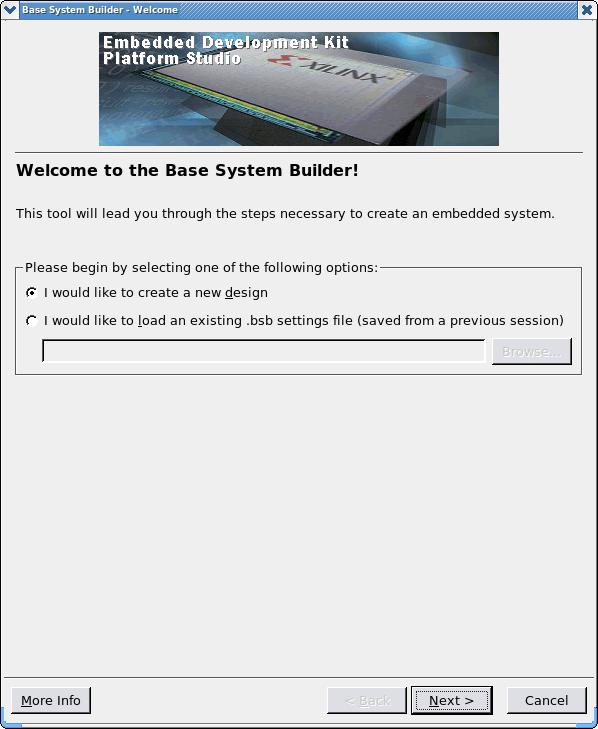
\includegraphics[scale=0.4]{BSB1}
\caption{Choose to create a new design. Click Next\label{fig:BSB1}}
\end{figure}
\begin{figure}[H]
\centering
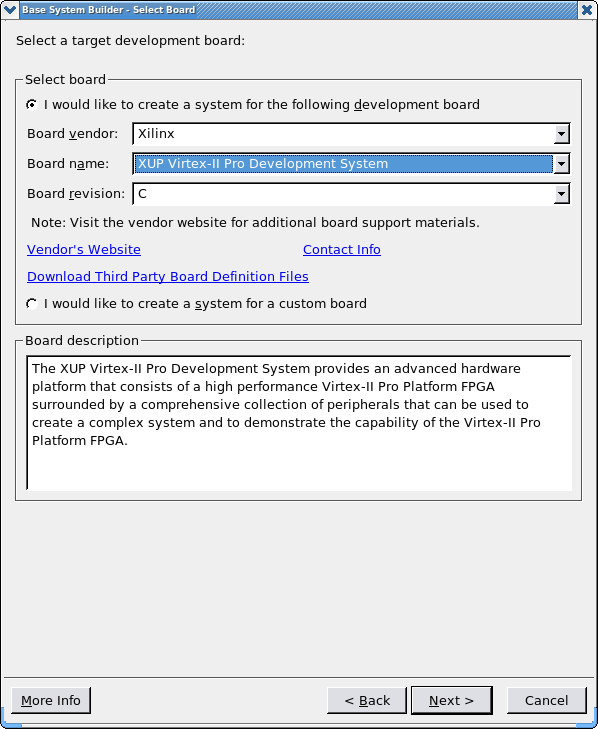
\includegraphics[scale=0.4]{BSB2}
\caption{Choose Xilinx as board vendor. Choose the XUP board. Click Next\label{fig:BSB2}}
\end{figure}
\begin{figure}[H]
\centering
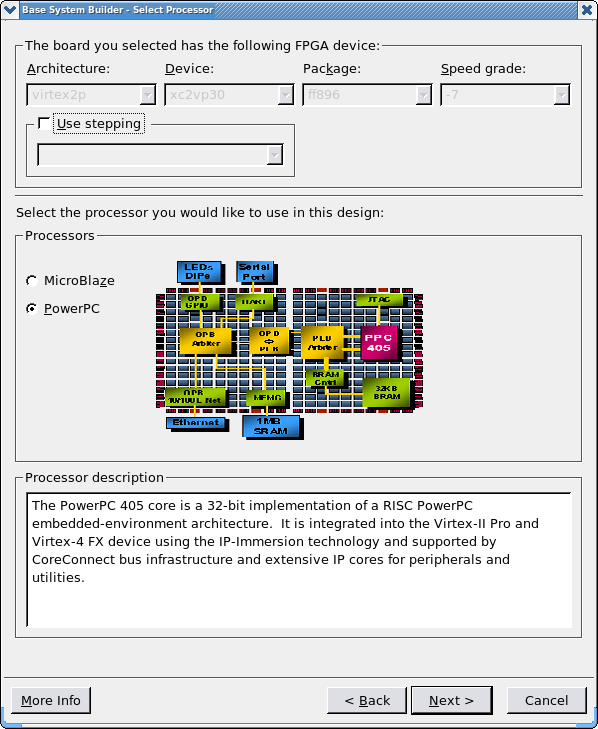
\includegraphics[scale=0.4]{BSB3}
\caption{Choose to use a the PowerPc. Click Next\label{fig:BSB3}}
\end{figure}
\begin{figure}[H]
\centering
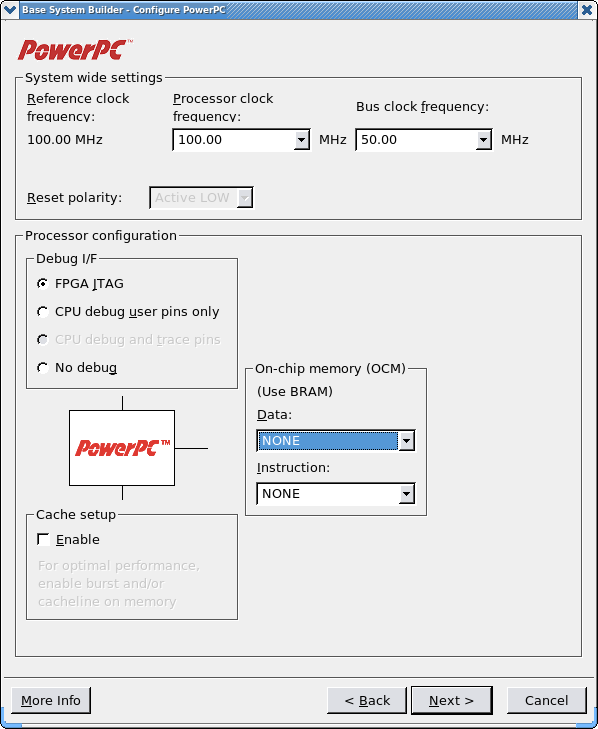
\includegraphics[scale=0.4]{BSB4}
\caption{Choose 50MHz as Bus Clock Frequency (The ICAP can maximally handle 66MHz). Click Next\label{fig:BSB4}}
\end{figure}
\begin{figure}[H]
\centering
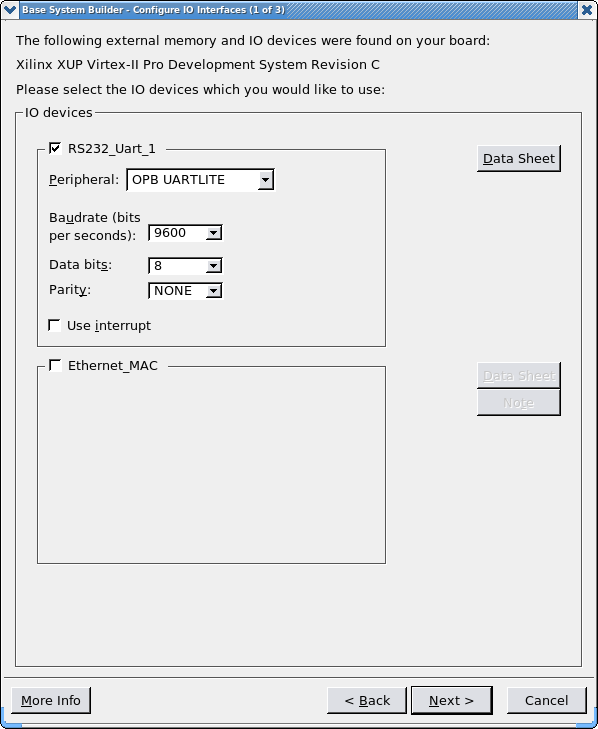
\includegraphics[scale=0.4]{BSB5}
\caption{Retain only the OPB\_UARTLITE in the next three windows\label{fig:BSB5}}
\end{figure}
%\begin{figure}[H]
%\centering
%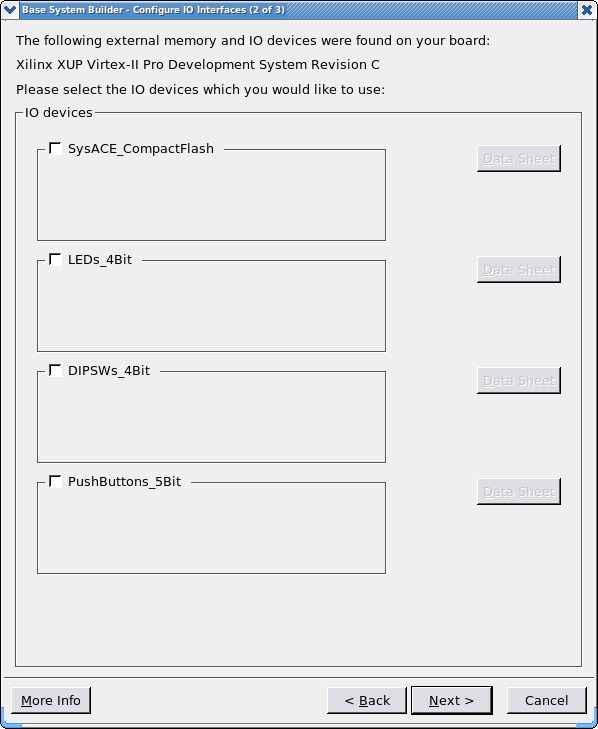
\includegraphics[scale=0.4]{BSB6}
%\caption{\label{fig:BSB6}}
%\end{figure}
%\begin{figure}[H]
%\centering
%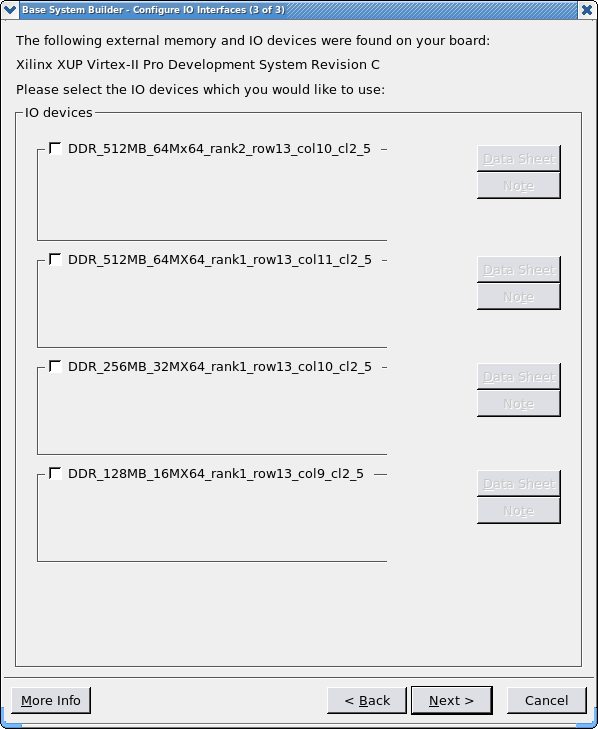
\includegraphics[scale=0.4]{BSB7}
%\caption{\label{fig:BSB7}}
%\end{figure}
\begin{figure}[H]
\centering
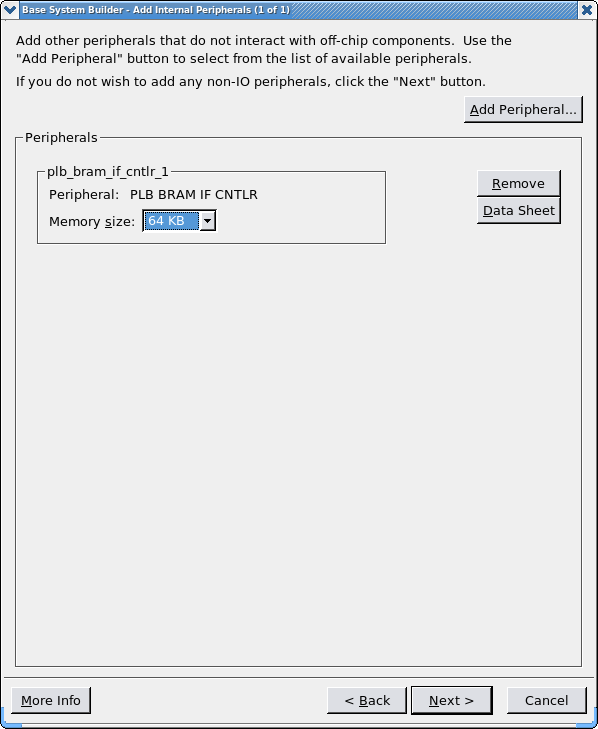
\includegraphics[scale=0.4]{BSB8}
\caption{Use 64kB of memory. Click Next\label{fig:BSB8}}
\end{figure}
\begin{figure}[H]
\centering
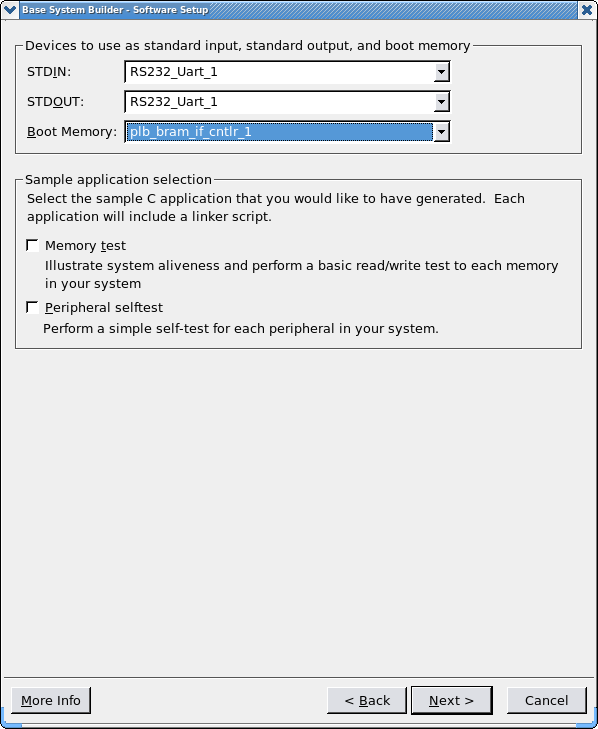
\includegraphics[scale=0.4]{BSB9}
\caption{Choose the UART as STDIN and STDOUT. Don't generate sample applications. Click Next\label{fig:BSB9}}
\end{figure}
\begin{figure}[H]
\centering
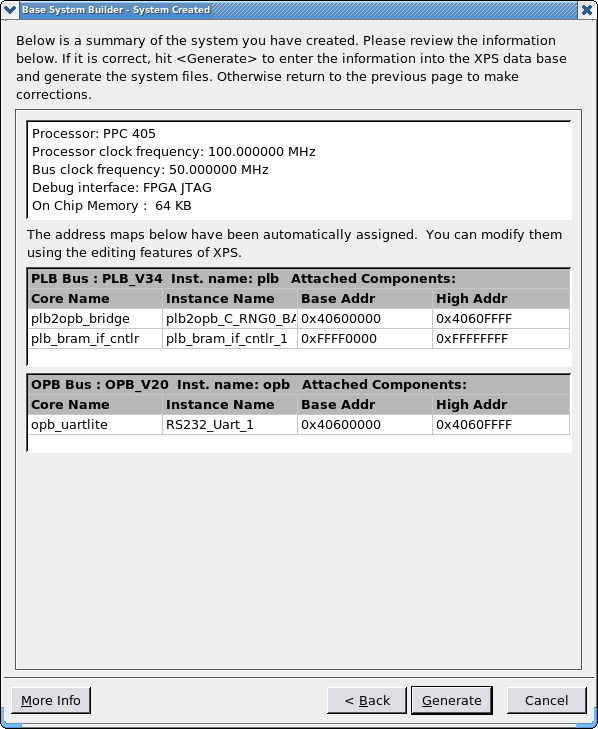
\includegraphics[scale=0.4]{BSB10}
\caption{Generate the project. Click Generate\label{fig:BSB10}}
\end{figure}
\begin{figure}[H]
\centering
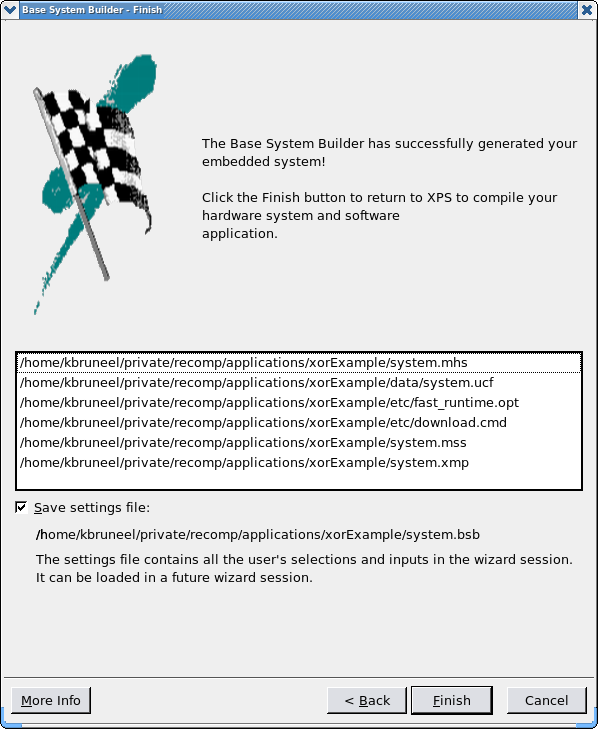
\includegraphics[scale=0.4]{BSB11}
\caption{Click Finish\label{fig:BSB11}}
\end{figure}


\subsection{Adding the HWICAP}\label{sec:adding_hwicap}
The HWICAP is used for run-time reconfiguration of the FPGA. This peripheral must be added to the project and connected to the OPB.
\begin{figure}[H]
\centering
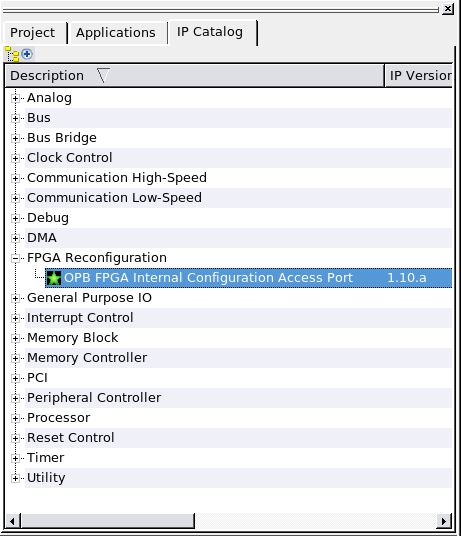
\includegraphics[scale=0.5]{HWICAP1}
\caption{In the IP Catalog, double click ``OPB FPGA Internal Configuration Access Port''. Click Yes\label{fig:HWICAP1}}
\end{figure}
\begin{figure}[H]
\centering
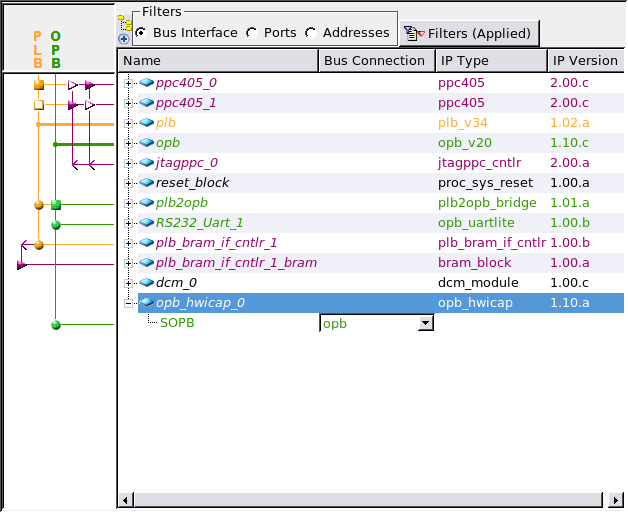
\includegraphics[scale=0.5]{HWICAP2}
\caption{An instance of the opb\_hwicap appears in the System Assembly View. Connect the hwicap to the OPB\label{fig:HWICAP2}}
\end{figure}
\begin{figure}[H]
\centering
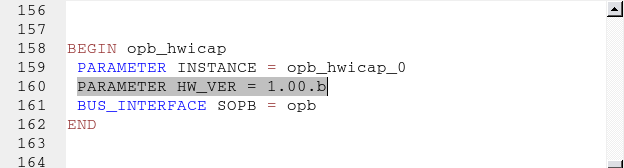
\includegraphics[scale=0.5]{HWICAP3}
\caption{Open the MHS file by double clicking it in the Project tab. Search the opb\_hwicap instance and change the version from \emph{1.10.a} to \emph{1.00.b}\label{fig:HWICAP3}}
\end{figure}
\begin{figure}[H]
\centering
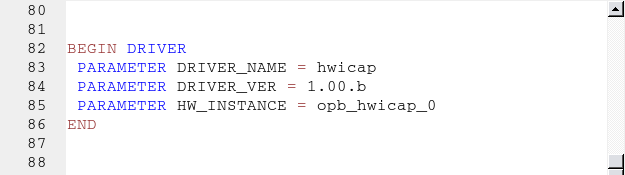
\includegraphics[scale=0.5]{HWICAP4}
\caption{Open the MSS file by double clicking it in the Project tab. Search the opb\_hwicap instance and change the version from \emph{1.01.a} to \emph{1.00.b}\label{fig:HWICAP4}}
\end{figure}

Finally, create a symbolic link in the directory `drivers' (create the directory if needed) of your project to `examples/xorExample/xps/drivers/hwicap\_v1\_00\_b'.


\subsection{Creating the DCS peripheral}\label{sec:creating_peripheral}
Currently, DCS can only be done on exactly one peripheral of the OPB bus. In this section you create this OPB peripheral with memory mapped registers.
\begin{figure}[H]
\centering
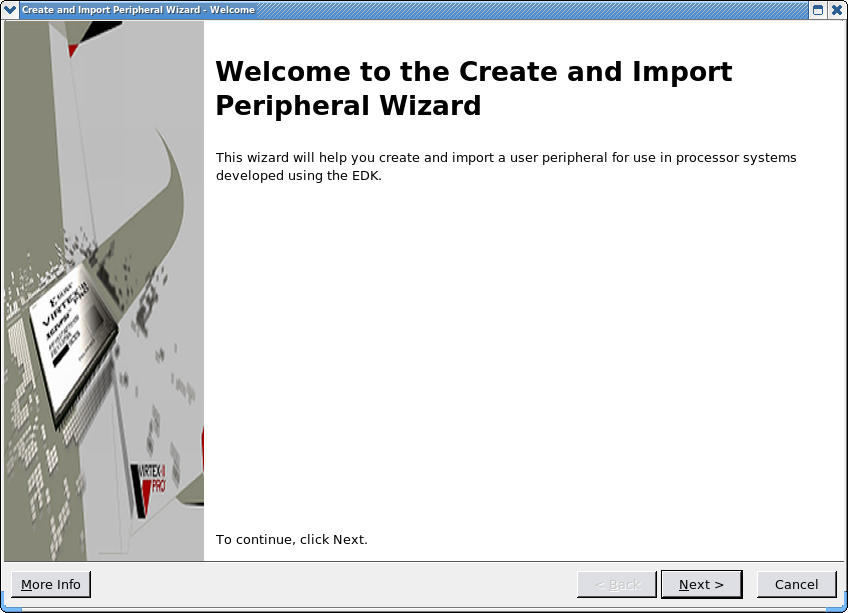
\includegraphics[scale=0.5]{COIP1}
\caption{Start the Create and Import Peripheral Wizard. Start the wizard from the Hardware menu. Click Next\label{fig:COIP1}}
\end{figure}
\begin{figure}[H]
\centering
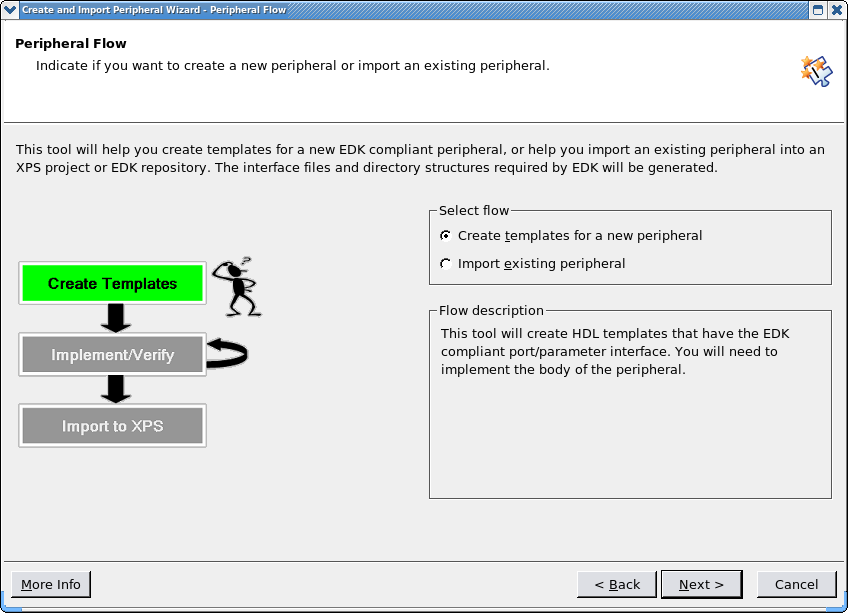
\includegraphics[scale=0.5]{COIP2}
\caption{Choose Create templates for a new peripheral. Click Next\label{fig:COIP2}}
\end{figure}
\begin{figure}[H]
\centering
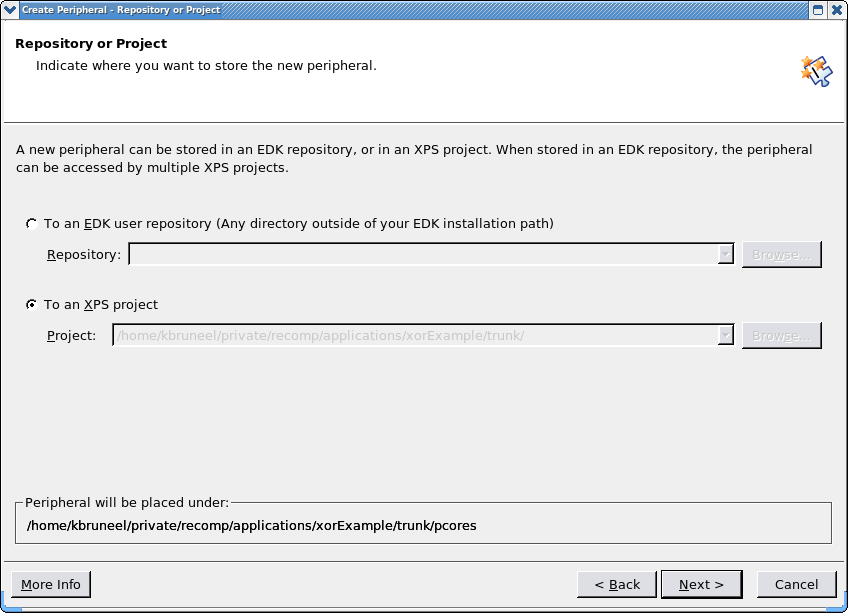
\includegraphics[scale=0.5]{COIP3}
\caption{Choose to store the peripheral in the XPS project. Click Next\label{fig:COIP3}}
\end{figure}
\begin{figure}[H]
\centering
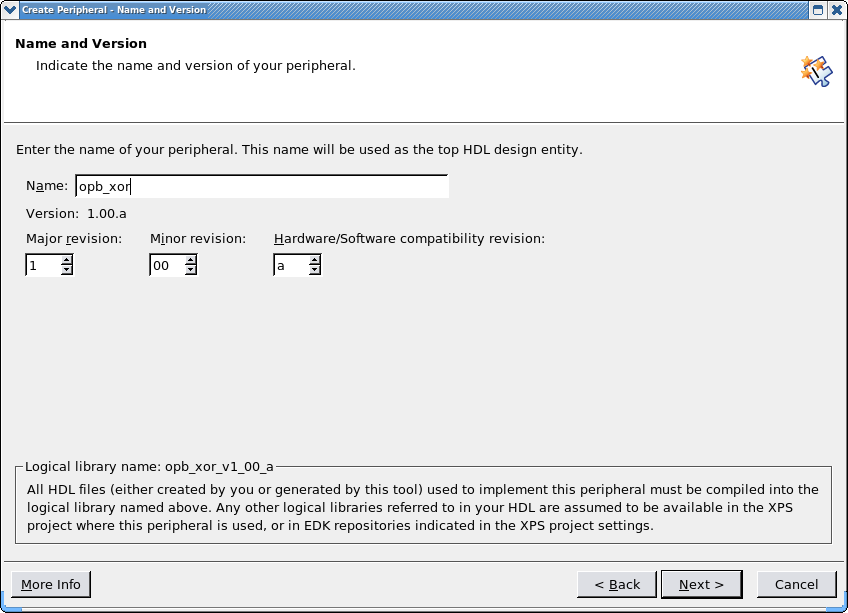
\includegraphics[scale=0.5]{COIP4}
\caption{Choose a name for the peripheral (E.g. `opb\_xor'). Click Next\label{fig:COIP4}}
\end{figure}
\begin{figure}[H]
\centering
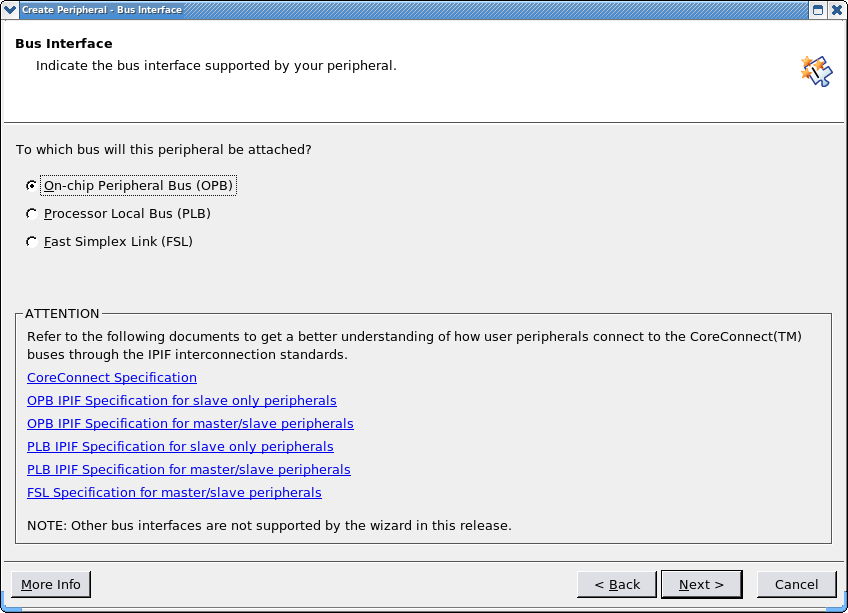
\includegraphics[scale=0.5]{COIP5}
\caption{Choose to create an OPB peripheral. Click Next\label{fig:COIP5}}
\end{figure}
\begin{figure}[H]
\centering
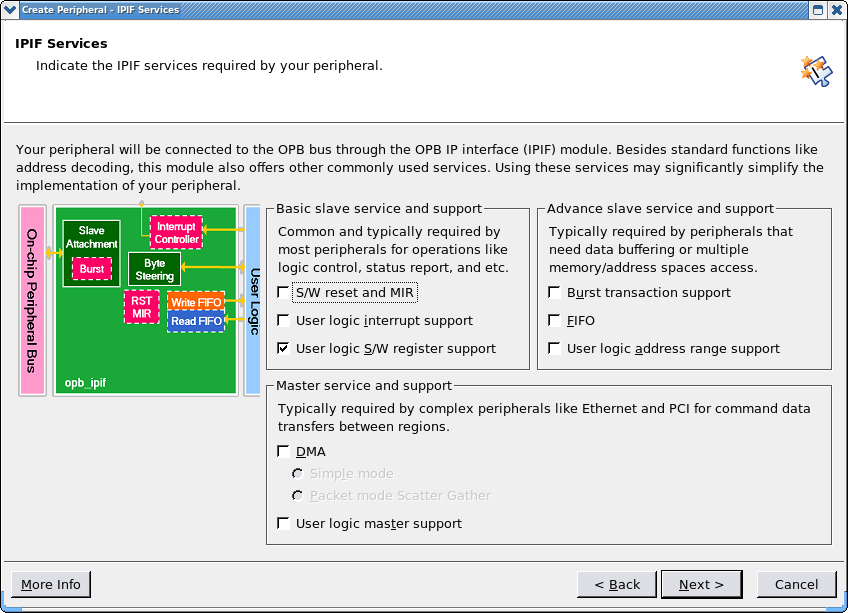
\includegraphics[scale=0.5]{COIP6}
\caption{Choose for User logic S/W register support deselect S/W reset and MIR. Click Next\label{fig:COIP6}}
\end{figure}
\begin{figure}[H]
\centering
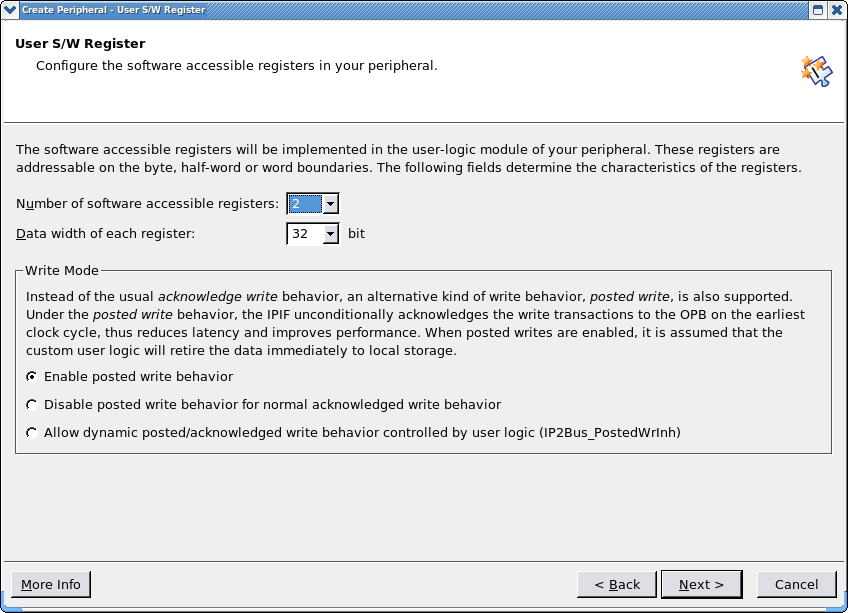
\includegraphics[scale=0.5]{COIP7}
\caption{Choose the required number and width of the registers. For the `xorExample' choose two 32-bit registers, one for the input and one for the output. Click Next\label{fig:COIP7}}
\end{figure}
\begin{figure}[H]
\centering
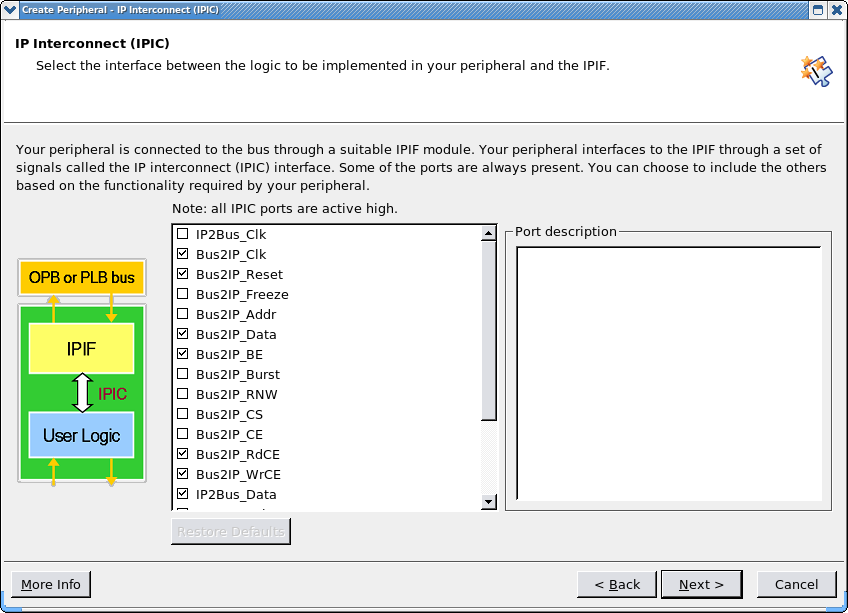
\includegraphics[scale=0.5]{COIP8}
\caption{Don't change anything. Click Next\label{fig:COIP8}}
\end{figure}
\begin{figure}[H]
\centering
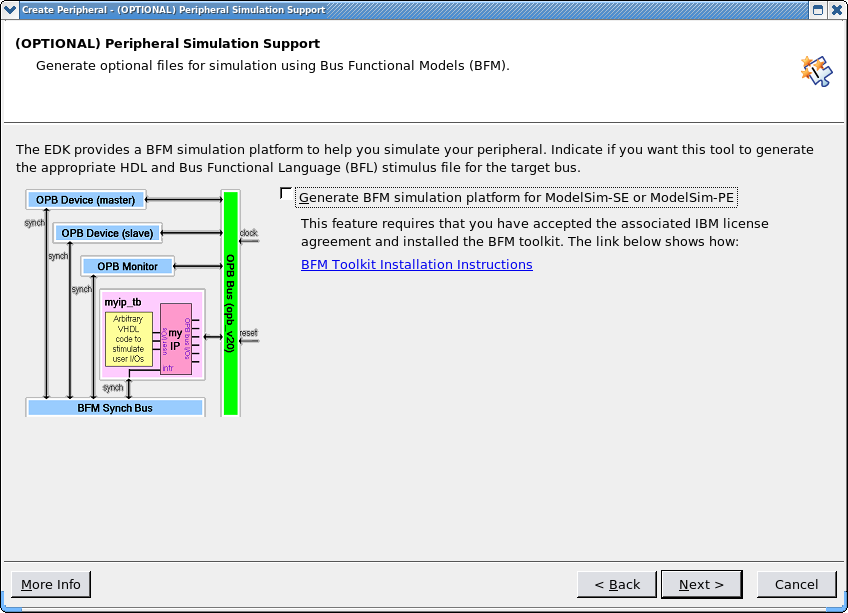
\includegraphics[scale=0.5]{COIP9}
\caption{Don't change anything. Click Next\label{fig:COIP9}}
\end{figure}
\begin{figure}[H]
\centering
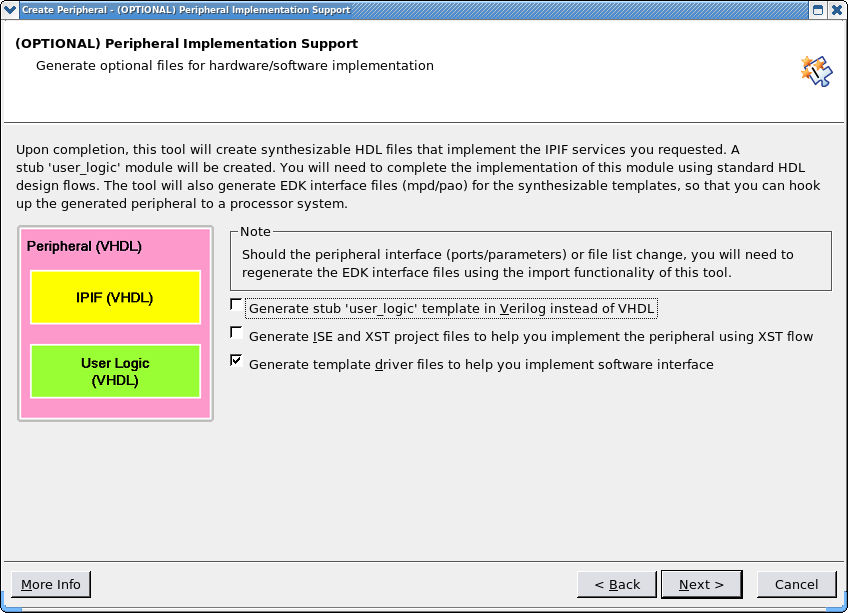
\includegraphics[scale=0.5]{COIP10}
\caption{Deselect Generate ISE and XPS project files. Click Next\label{fig:COIP10}}
\end{figure}
\begin{figure}[H]
\centering
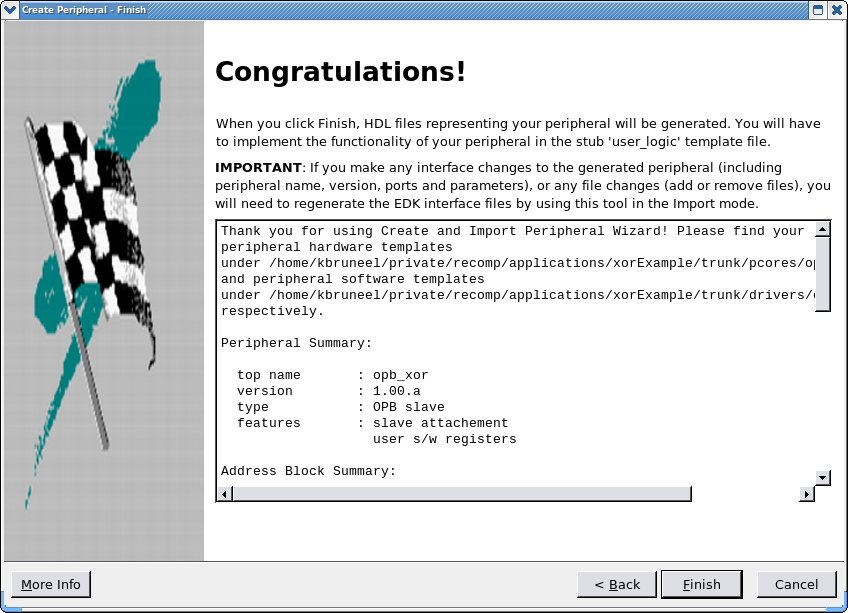
\includegraphics[scale=0.5]{COIP11}
\caption{Click Finish\label{fig:COIP11}}
\end{figure}

\subsection{Adding the DCS peripheral}\label{sec:adding_peripheral}
\begin{figure}[H]
\centering
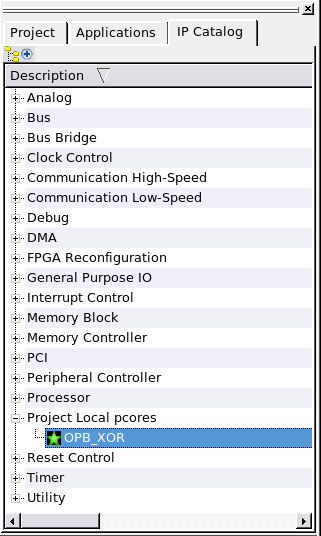
\includegraphics[scale=0.5]{AXOR1}
\caption{In the IP Catalog, double click your OPB peripheral (E.g. `OPB\_XOR'). Click Yes.\label{fig:AXOR1}}
\end{figure}
\begin{figure}[H]
\centering
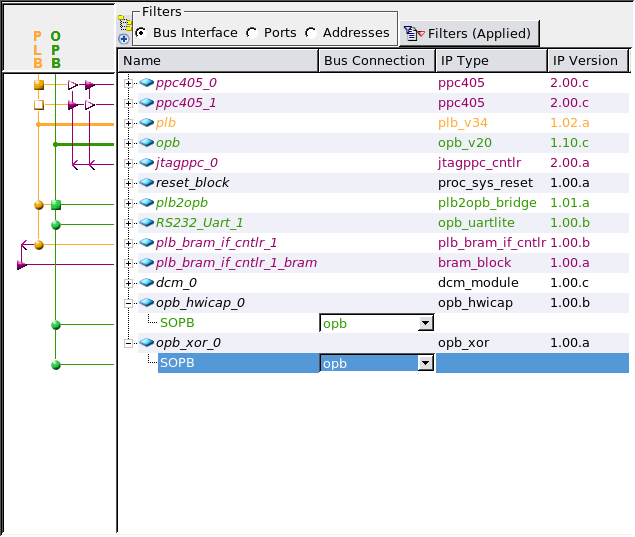
\includegraphics[scale=0.5]{AXOR2}
\caption{An instance of the peripheral appears in the System Assembly View. Connect the peripheral to the opb\label{fig:AXOR2}}
\end{figure}
\begin{figure}[H]
\centering
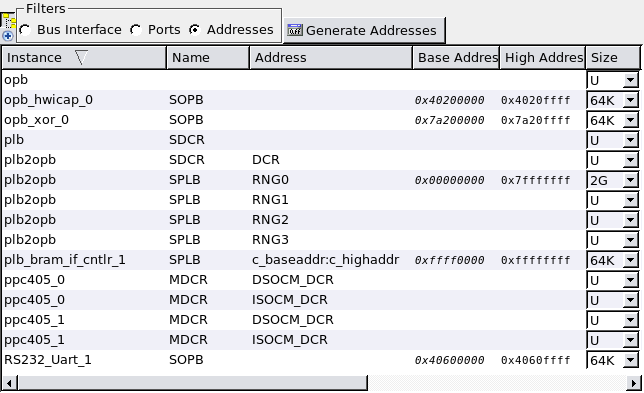
\includegraphics[scale=0.5]{AXOR3}
\caption{Select the Addresses view in the System Assembly View. Click the Generate Addresses button\label{fig:AXOR3}}
\end{figure}


\subsection{Creating the software application}\label{sec:creating_software}
\begin{figure}[H]
\centering
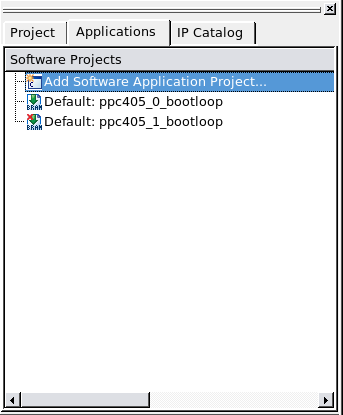
\includegraphics[scale=0.5]{soft1}
\caption{Double Click ``Add Software Application Project\dots'' in the Applications tab\label{fig:soft1}}
\end{figure}
\begin{figure}[H]
\centering
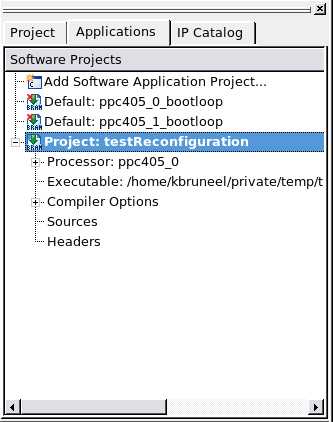
\includegraphics[scale=0.5]{soft2}
\caption{Right click  on the project. Click ``Mark to Initialize BRAMs'' in the pop down menu. Also unmark ppc405\_0\_bootloop\label{fig:soft2}}
\end{figure}


\subsection{Creating the custom makefile}\label{sec:creating_makefile}
\begin{itemize}
\item Choose  ``Generate netlist''. You may immediately terminate it once started.
\item Copy `system.make' to `custom.make' in your project directory.
\item In `custom.make', add the line ``include tmap.make'' right after ``include system\_incl.make''.
\item Click ``Project Options...'' in the ``Project'' menu and choose `custom.make' as the Custom Makefile (Figure~\ref{fig:makefile}).
\end{itemize}
Make sure that you  copy `system.make' after creating the software application. Do this again when you add new software applications.
\begin{figure}[H]
\centering
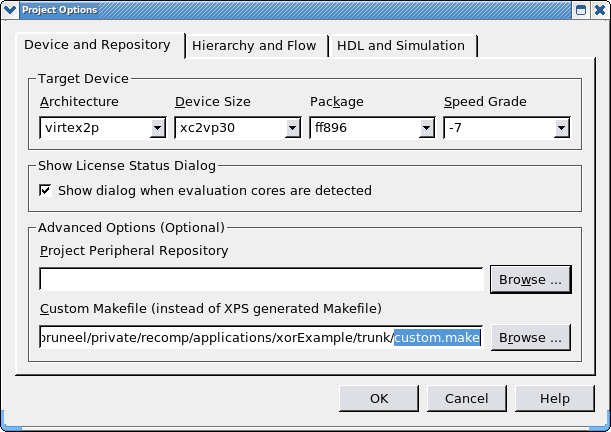
\includegraphics[scale=0.5]{make}
\caption{Choose `custom.make' as the Custom Makefile. Click Ok\label{fig:makefile}}
\end{figure}



\subsection{Writing the DCS peripheral}\label{sec:writing_peripheral}
\begin{itemize}
\item Go to the subdirectory corresponding to your DCS peripheral in the `pcores' directory of the project.
\item Copy the `hdl/vhdl' directory to the `design' directory. It should contain two files `opb\_<peripheral\_name>.vhd' and `user\_logic.vhd'.
\item Add the VHDL code of your DCS design to the `design' directory. It is advised that you run your design through the standalone TLUT tool flow first (Section\ \ref{sec:standalone_flow}). Add the line `-\--TMAP' to the top of the file that you want to perform DCS on. This does not have to be the top level module of the peripheral.
\item Add the names of your VHDL modules to the `.pao' file in the `data' directory. Modules that are only used as a submodule of your DCS module should not be included. Note that if a module depends on another module it should be listed after it.
\item Add the line ``OPTION CORE\_STATE = development'' to the `.mpd' file in the `data' directory to ensure that your peripheral is synthesized again if changes are made to it.
\item Instantiate your module in the architecture description of `user\_logic.vhd' and connect the inputs and outputs to the memory-mapped registers of the OPB peripheral. Assign the parameter inputs a dummy value.\\
E.g. for  `xorExample':
\lstset{language=VHDL}
\begin{lstlisting}
EXORS: entity work.exorw32
port map (
     a => slv_reg0,
     x => slv_reg1,
     p => (others => '0')
);
\end{lstlisting}
\item Remove the write functionality for read-only registers. For the `xorExample',  `slv\_reg1' is read-only (Figure~\ref{fig:design1}).
\begin{figure}[H]
\centering
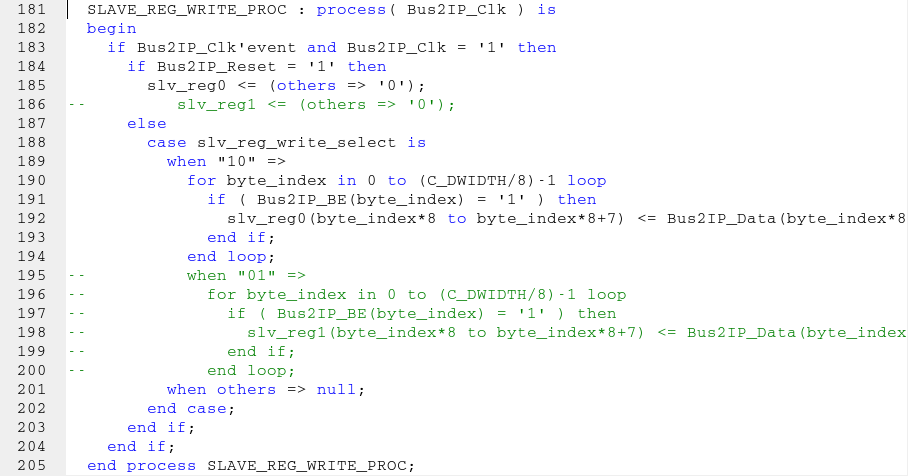
\includegraphics[scale=0.5]{design1}
\caption{Removing the write functionality for read-only registers\label{fig:design1}}
\end{figure}
\item Enter the `design' directory and run `generateTMAPMake.py'. This creates the custom makefile `tmap.make'. You have to rerun `generateTMAPMake.py' if you add files to the DCS peripheral or change the `-\--TMAP' annotation.
\item Choose ``Generate bitstream'' in XPS to build your peripheral.
\item Look near the end of the output of this command for ``Group path: '' followed by something similar to ``opb\_xor\_0/opb\_xor\_0/USER\_LOGIC\_I/EXORS/*''.
Edit `data/system.ucf' and add the following lines before the IO constraints, replacing <group\_path> with the path found before. Increase the range of the group as needed. This area constraint makes sure that  run-time reconfiguration does not break the rest of your design by accidentally resetting BRAMs.

\lstset{language=}
\begin{lstlisting}
INST "<group_path>" AREA_GROUP=group1;
AREA_GROUP "group1" COMPRESSION=0;
AREA_GROUP "group1" RANGE=SLICE_X0Y*:SLICE_X51Y*;
\end{lstlisting}


\end{itemize}

\subsection{Writing the software application}\label{sec:writing_software}
\begin{itemize}
\item Choose ``Generate bitstream'' if you haven't already done this. This will create a number of C files in `testReconfiguration' that  contain the functions needed to perform run-time reconfiguration.
\item Under the applications tab, right click ``Sources'' and choose ``Add existing files\dots''. Add `testReconfiguration/locations.c' and `testReconfiguration/<TMAPmodule>.c' with TMAPmodule the name of the VHDL module that has the ``-\--TMAP'' annotation.
\item Right click ``Headers'' choose ``Add existing files\dots''. Add `testReconfiguration/locations.h' and `testReconfiguration/<TMAPmodule>.h'.
\item Right click ``Sources'' and choose ``Add new file\dots''. Call it `main.c' and save it.\\
You can find a template for your `main.c' file below or at the bottom of `testReconfiguration/<TMAPmodule>.h'. Replace ``XPAR\_OPB\_XOR\_0\_BASEADDR'' with the name of the base address of your peripheral. You can find this in `Generated Header: ppc405\_0/include/xparameters.h' under  `Processor: ppc405\_0'.
\item Choose ``Build all user applications'' to build your software application.
\end{itemize}

\lstset{language=[ansi]C,showstringspaces=false}
\begin{lstlisting}
#include "<TMAPmodule>.h"

int main(void) {
	xil_printf("Starting EXOR test...\n\r\n\r");
	//Initialization
	static XHwIcap HwIcap;
	XHwIcap_Initialize(&HwIcap, HWICAP_DEVICEID, XHI_TARGET_DEVICEID);
	//Run-time reconfiguration
	Xuint8 i;
	Xuint8 parameter[NUMBER_OF_PARAMETERS];
	Xuint8 output[NUMBER_OF_INSTANCES][16];
	xil_printf("Configuring the LUTs for p=0...\n\r");
	for (i=0;i<NUMBER_OF_INSTANCES;i++) {
		//Reconfigure one instance
		parameter[0]=0;
		evaluate(parameter,output);
		reconfigure(&HwIcap,output,location_array[i]);
	}
	xil_printf("Configuration Complete!\n\r\n\r");
	//Testing configuration
	xil_printf("Writing 0xDEADBEAF to input register...\n\r");
	XIo_Out32(XPAR_OPB_XOR_0_BASEADDR,0xDEADBEAF);
	xil_printf("Reading output register: %x\n\r\n\r", 
		XIo_In32(XPAR_OPB_XOR_0_BASEADDR+4));
	xil_printf("End EXOR test.\n\r\n\r");
	return 1;
}
\end{lstlisting}

Explanation of the functions:\\
$evaluate(parameter, output)$ calculates the new truth table contents of the TLUTs for the new values of the parameters. The  values of the parameter signals have to be stored as boolean values in the $parameter$ array (one array element per signal line). The parameters are sorted alphabetically. You can check this ordering in `pcores/opb\_<your\_peripheral>/design/work/<TMAPmodule>.par'.\\
$reconfigure(\&HwIcap, output, location\_array[i])$ reconfigures the TLUTs of instance $i$ with the previously computed truth table contents. The instances are also sorted alphabetically. You can find this ordering in `testReconfiguration/locations.c'.


\subsection{Testing the design}\label{sec:testing}
The project can now be tested. To do this, connect your XUPV2P board to the computer using a USB cable (for bitstream programming) and a serial cable (for debugging). Start the program minicom to read the debug output from your XUPV2P board. Then, choose ``Download bitstream'' in XPS to run your project on the FPGA.


\section{Troubleshooting}\label{sec:xilinx_troubleshooting}
It is assumed that you have already successfuly run the tests for the standalone TLUT tool flow (Section~\ref{sec:standalone_flow}).

\begin{itemize}
\item \emph{Throws ``tmap.py: Command not found'':}\\
Make sure you have set the environment variables correctly by doing `. source'. You must do this in the same terminal as you start XPS in and before starting XPS.
\item \emph{The output of minicom is garbage:}\\
Reboot your computer to fix the corrupted state the serial port is in. The corrupted state may be caused by running minicom and `virtex2pro\_test.sh' at the same time.
\item \emph{Reconfiguration does not happen, even for the example designs:}\\
Check the jumper settings of the XUPV2P board.
\end{itemize}



\clearpage
\chapter{Contents}\label{sec:contents}
The `tlut\_flow' folder contains a number of folders and three files: `Makefile', `README.md' and `LICENSE'. 
The `Makefile' is used to initially set up the tool flow. It will download  some necessary third party tools and compile the used programs.
More information about the license under which the TLUT tool flow is released can be found in `LICENSE'.\\

The `tlut\_flow' folder contains the following folders:  `examples', `tests', `documentation',  `java', `python' and `third\_party'.

\begin{itemize}
\item In the `examples' folder you can find a number of designs that use the TLUT tool flow. You can run each of them by executing the Python script contained in the respective subfolder. You can run all examples at once (except AES) by executing the `run\_all.sh' script.
\item In the `tests' folder you can currently find one test, namely `examples\_test.sh'. Executing this script will run the `examples/run\_all.sh' script and compare the output to the expected output.
\item The `documentation' folder contains this document, and its Latex source files, and the Ph.D. thesis by Karel Bruneel which contains more information about the academic underpinnings of the TLUT tool flow.
\end{itemize}

The remaining folders contain binaries, source code and wrapper scripts. You may want to edit these when doing advanced experiments.
\begin{itemize}
\item The `java' folder contains the Java source and binary files of a simple technology mapper and an adapted parameterized version of this technology mapper, the TLUT technology mapper.
\item After setup, the `third\_party' folder will contain ABC, the logic synthesis and technology mapping tool of the university of Berkeley, and Aiger, a tool used to handle textual (.aag) and binary representations of and-inverter-graphs (.aig).    

\item The `python' folder contains the high level Python scripts that are used to interface with the tools in the other folders. It contains three files: `fast\_tlutmap.py', `genParameters.py' and `mapping.py'. The `genParameters.py' script will extract the parameters from the annotated VHDL file. The `mapping.py' script contains high level wrappers that call the different mappers and a number of utility programs. These 2 last scripts are best used as given. 

The `fast\_tlutmap.py' script contains the main code in the `run' function. This function can easily be adjusted to meet the user's needs. The run function mainly consists of 2 steps: synthesis and technology mapping. The synthesis step converts the VHDL file into a logic circuit in blif format using Quartus II. The technology mapping step will map the logic circuit to a circuit with LUTs. Three different technology mapping tools are included to allow an easy comparison: the simple mapper, the TLUT technology mapper and the ABC mapper. The first two are not as optimized as ABC. For example `area recovery' is not yet completely implemented. The ABC tool flow is an academic framework that does include a large number of such optimizations. Several commercial tools are based on this technology mapper.

The `run' function also contains some intermediate steps:
\begin{itemize} 
\item the conversion of the blif format into the aag format, needed for the Java mappers
\item extraction of the parameters out of the annotated VHDL file
\end{itemize}

\end{itemize}

%Hier zouden ook nog alle voorbeelden moeten beschreven worden, vanaf welke formaat ze starten (vhdl, verilog, aag) en een zin over wat ze moeten voorstellen.



\end{document}
